\begin{activity}{Thermal Refraction in Layered Crustal Rocks}

\section*{Purpose}
To explore thermal refraction caused by conductivity contrasts within the crust, particularly in sedimentary and metamorphic layering.

{\color{red}
\section*{Learning Outcomes}

By the end of this activity, you should be able to:
\begin{itemize}
  \item Describe how alternating high- and low-conductivity layers create systematic variations in the temperature gradient at constant heat flow.
  \item Sketch a temperature--depth profile through a sequence of alternating shale and quartzite layers.
  \item Explain how tilted layering distorts isotherms and creates lateral heat flow components.
  \item Connect layered conductivity anisotropy to the mixing law concepts introduced in Week~2.
\end{itemize}
}

\section*{Geological Context}
Many crustal sections contain cyclic layering inherited from sedimentary environments, such as alternating shales and quartz-rich sandstones that later become quartzites.

\begin{itemize}
  \item Shales: low thermal conductivity.
  \item Quartzites: high thermal conductivity.
\end{itemize}

This layering can persist through burial, deformation, and metamorphism.

\section*{Tasks}
\begin{enumerate}
  \item Consider a vertical sequence of alternating shale and quartzite layers.
  Assume constant heat flow through the sequence. Sketch the layer sequence and label the conductivities.
  \answerbox[3cm]

  \item Using
  \[
    q = -k \nabla T,
  \]
  explain how the temperature gradient differs in shale layers compared to quartzite layers.
  \answerbox[3cm]

  \item Sketch a qualitative temperature--depth profile showing changes in slope across layers.
  \answerbox[5cm]

  \item Now consider the same layered sequence tilted relative to vertical heat flow. Describe how thermal refraction will distort isotherms.
  \answerbox[3cm]
\end{enumerate}

\section*{Extension}
\begin{itemize}
  \item How can cyclic layering create an effectively anisotropic thermal conductivity?
  \answerbox[3cm]
  \item How might folding or tilting further modify the thermal field?
  \answerbox[3cm]
\end{itemize}

\section*{Connection}
Relate this behavior to the physical-properties mixing demonstrations discussed earlier in the course.

\answerbox[3cm]

{\color{red}
\section*{Key Ideas}

{\color{blue}
\textbf{Cyclic layering creates effective thermal anisotropy.} A sequence of alternating low- and high-conductivity layers has different effective conductivities depending on whether heat flows parallel or perpendicular to the layers --- the harmonic mean (perpendicular) is always less than the arithmetic mean (parallel). This is exactly the mixing law behaviour explored in Week~2.

\begin{figure}[h]
\centering
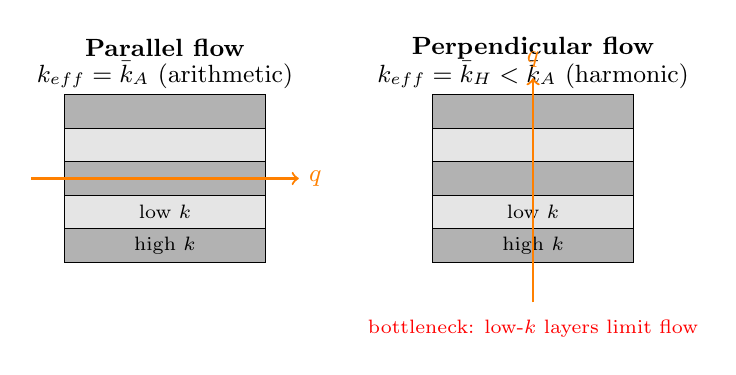
\begin{tikzpicture}[scale=0.85]
  % --- Parallel flow (arithmetic mean) ---
  \node[font=\small\bfseries] at (1.5, 3.2) {Parallel flow};
  \node[font=\small] at (1.5, 2.8) {$k_\text{eff} = \bar{k}_A$ (arithmetic)};
  % Layers (horizontal)
  \foreach \y/\col in {0/gray!60, 0.5/gray!20, 1.0/gray!60, 1.5/gray!20, 2.0/gray!60} {
    \fill[\col] (0,\y) rectangle (3, \y+0.5);
    \draw (0,\y) rectangle (3, \y+0.5);
  }
  \node[font=\scriptsize] at (1.5, 0.25) {high $k$};
  \node[font=\scriptsize] at (1.5, 0.75) {low $k$};
  % Heat flow arrow (horizontal = parallel to layers)
  \draw[->, thick, orange] (-0.5, 1.25) -- (3.5, 1.25) node[right, font=\small] {$q$};

  % --- Perpendicular flow (harmonic mean) ---
  \node[font=\small\bfseries] at (7.0, 3.2) {Perpendicular flow};
  \node[font=\small] at (7.0, 2.8) {$k_\text{eff} = \bar{k}_H < \bar{k}_A$ (harmonic)};
  % Same layers
  \foreach \y/\col in {0/gray!60, 0.5/gray!20, 1.0/gray!60, 1.5/gray!20, 2.0/gray!60} {
    \fill[\col] (5.5,\y) rectangle (8.5, \y+0.5);
    \draw (5.5,\y) rectangle (8.5, \y+0.5);
  }
  \node[font=\scriptsize] at (7.0, 0.25) {high $k$};
  \node[font=\scriptsize] at (7.0, 0.75) {low $k$};
  % Heat flow arrow (vertical = perpendicular)
  \draw[->, thick, orange] (7.0, -0.6) -- (7.0, 2.75) node[above, font=\small] {$q$};
  \node[font=\scriptsize, red] at (7.0, -1.0) {bottleneck: low-$k$ layers limit flow};
\end{tikzpicture}
\caption{Layered anisotropy: heat flowing parallel to layers uses the arithmetic mean conductivity; heat flowing perpendicular is limited by the harmonic mean (controlled by low-conductivity layers).}
\end{figure}
}

\textbf{Tilted layers redirect heat.} When conductivity contrasts are tilted relative to the heat flow direction, a component of heat flow is deflected laterally. Isotherms are no longer horizontal; they arch upward over high-conductivity regions and downward over low-conductivity regions.

\textbf{Structural geology affects the thermal field.} Folding, thrusting, or tilting of conductivity contrasts can create significant lateral temperature variations even in a regionally uniform heat-flow setting. This complicates heat-flow measurements and must be accounted for in geothermal assessments.
}

\end{activity}